\begin{figure}
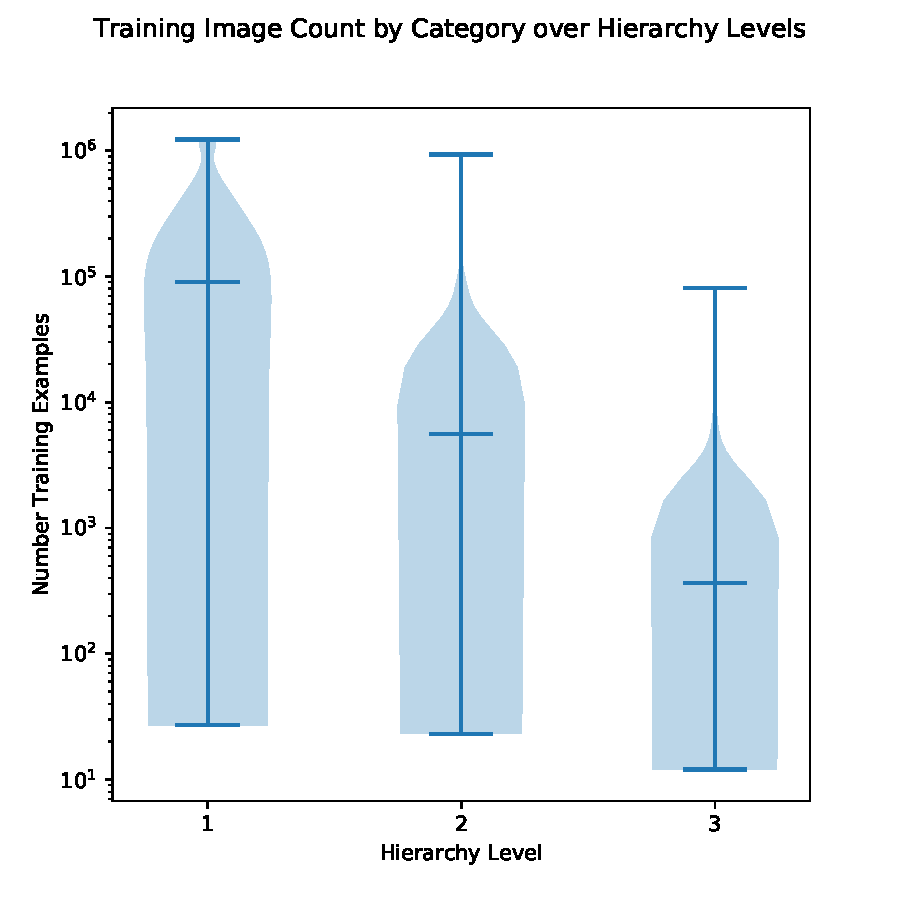
\includegraphics[width=\columnwidth]{img/datacount}
\caption{
This violin plot compares the number of training examples available for first (top) level categorizations, second level categorizations, and third (bottom) level categorizations.
As would be expected, the median training data count is highest for first level categories and lowest for third level categories.
On all three hierarchical levels, training data is distributed unevenly between categories.
For example, although the median top level category has approximately $10^5$ training examples, some have fewer than 100.
In all three subplots, horizontal bars mark the 0, 50, and 100th percentile counts.
}
\label{fig:datacount}
\end{figure}